\chapter{Results}
\label{c:results}

This chapter presents the main results in a logical succession, corresponding with the objectives defined in the \nameref{s:intro:need-for-transition} section. The development of the vision of a future sustainable mobility system is given in \autoref{s:results:ssp1-mob}. In \autoref{s:results:backcasting-ssp1-mob}, this vision is used as the basis of a backcasting process to determine the necessary changes to achieve the sustainable mobility paradigm. \autoref{s:results:autolock-model} presents a conceptual model to build insights on the current state of the automobility system with respect to its dynamics of change and stability. These dynamics are put in opposition to the necessary changes derived in the backcasting process, to discuss long-term policy recommendations in \autoref{s:results:policy-recommendations}.

\section[SSP1-MOB sustainable mobility scenario]{SSP1-MOB: a mobility extension of a sustainable development scenario}
\label{s:results:ssp1-mob}
In order to develop a future vision that tells us how mobility is conceived in the year 2100, two main options are available: (a) write and justify a new vision from the ground up or (b) building upon already developed visions found throughout the literature. Both to reduce the time spent on this task and to increase the legitimacy\footnote{Given that no participatory process is carried to describe or develop the future vision and the corresponding backcasting, expert opinions, in the form of widely accepted scientific scenarios, are used.} of the result, the second option is chosen. \ssref{ss:results:ssp-scenarios-candidate} deals with the selection of the scenario that forms the basis of the future mobility vision, which is actually developed in \ssref{ss:results:ssp1-mob-development}. Finally, a discussion of the vision follows in \ssref{ss:results:ssp1-mob-paradigm}, contrasting the narrative to other results found in the literature.

\subsection{The SSP scenarios and the selected candidate}
\label{ss:results:ssp-scenarios-candidate}
The \gls{IPCC} has recently developed several scenarios that are the basis of their integrated climate change assessments \parencite{oneill2017_roadsaheadNarratives,vuuren2017_Energylanduse,fricko2017_markerquantificationShared,fujimori2017_SSP3AIMimplementation,calvin2017_SSP4worlddeepening,kriegler2017_Fossilfueleddevelopment}. These scenarios are called \glspl{SSP} and are defined on the basis of \emph{qualitative narratives} that contain all the necessary information on global trends to enable a further quantification step, using \glspl{IAM}, such as the IMAGE model \parencite{vuuren2017_Energylanduse}. Given that SSPs are not designed solely for the purpose of climate change studies, but are rather a description of world futures, they can be used in other disciplines and, particularly, in any kind of sustainability studies \parencite{oneill2017_roadsaheadNarratives}. Furthermore, the fact that the scenarios are developed in the form of a \emph{narrative} actually makes them closer to the concept of a ``vision'' than that of a traditional scenario: SSPs define final states, rather than trends or forecasts.

Among the five IPCC \gls{SSP} scenarios\footnote{The original narratives of all SSP1, SSP2, SSP3, SSP4 and SSP5 scenarios and the explanation of the assumptions taken to develop them can be found in \textcite{oneill2017_roadsaheadNarratives}.}, SSP1 ``\textit{Sustainability -- Taking the green road}'' is the one that implies a lower level of both adaptation and mitigation challenges with respect to climate change. Moreover, it is the one that is more aligned with the concept of Sustainable Development, due to its relatively high performance in all three pillars of sustainability: environmental conservation, social and economic sustainability (at least, economic \emph{growth} per capita). Therefore, it is the selected SSP to extend by covering the mobility sector, in order to perform the backcasting process that will be used in \sref{s:results:backcasting-ssp1-mob} to identify the necessary changes and development goals to reach a sustainable transport system in the future. The extension of the scenario, developed as a qualitative narrative is called \emph{SSP1-MOB}, from here on.

\subsection[The SSP1 mobility extension]{The SSP1 mobility extension: a narrative for the sustainable future}
\label{ss:results:ssp1-mob-development}
A particular \emph{vision} of a future sustainable mobility system is outlined in SSP1-MOB. Note that it is not comprehensive description of the myriad of elements composing the system, because it would not be feasible and too many sources of uncertainty would be introduced. Rather, it deals with travel patterns and which travel modes are most common, provided the necessary elements and configurations that make these patterns possible. To understand the frame of this narrative, it is \textbf{highly suggested} to read the original SSP1 storyline, which SSP1-MOB extends, reproduced in \aref{a:ssp1-original-narrative}. The following is the narrated version of SSP1-MOB, describing the global situation of the mobility system in the year 2100:
%
\blockquote{\sffamily \textbf{SSP1-MOB narrative (2100)}\\Driven by an increasing level of awareness of the environmental and socio-economic impacts of the transportation system, the world has adopted a series of changes throughout the decades to reduce those. Technology-wise, vehicles have become more efficient and liquid hydrocarbon fuels are less carbon intensive and renewable (based on biofuels). More importantly, though, there has been a major shift in travel modes and, most importantly, total travel demand per capita has been reduced. However, the global absolute total demand has increased, due to economic growth and increases in the living standard of countries in Africa, Asia and South America.

An increase in urban density (1st), a change in land use patterns (2nd) and a de-centralisation of economic development hotspots (3rd) are at the core of the substantial change in travellers' needs and, thus, behaviour. More concentrated urban centres allow for a shortening of trip lengths, up to a point where cycling and walking are feasible alternatives. The size of cities, however, is kept below certain thresholds that permit, in principle, for a more livable and sustainable way of life. This indeed means that a de-centralisation process has taken place, from huge, unwieldy metropolis to medium-sized cities, allowing for (and requiring) a more horizontal economic and governance structure. Moreover, there has been a generalised backlash against single-use urban development, this is, there has been a move towards mixing cultural, residential, work, institutional and commercial uses of the built environment. This form of urban development acknowledges the limitations of single-use schemes, such as isolation and automobility dependence. These de-centralisation and mixing trends allow people to avoid the need for relocation to find a job or, for the same matter, commute long distances. Instead, short to medium distances and travel times are the norm when commuting, thus preventing the further need and use of automobiles.

High education levels, widespread access to fast internet and changes in consumption patterns also contribute to lower travel demand. Teleworking is increasingly adopted by companies and in other office-based jobs, allowing people to work from shared co-working facilities that are near home or to avoid commuting altogether. IT access also facilitates the spread of information systems to make car sharing, carpooling and, most importantly, intermodal travel possible (and feasible) --- users can access and use travel information to plan their routes easily, reducing both travel time and cost. Less travel intensive consumption patterns have emerged, such as a reduction in long distance tourism. Due to the fact that common consumption objects, such as food and other amenities can be found within the local area, the need to travel far away has been reduced.

When it comes to travel mode alternatives, most of the demand is supplied through public transport, be it in the form of passenger rail, buses or aviation. An increased and continuous heavy investment in public transport infrastructure (an extensive railway network, for example) has enabled fast, secure and low-carbon transport options for the majority of the population, which lives in more concentrated urban areas. High speed trains cover the demand for regional and national trips and even international trips (whenever the distance is not excessive). Regular electric trains and trams are the main mode of transport for interurban commuters and travellers. For less accessible areas, efficient, bio-fuelled, hybrid and electric buses are used. Fast and reliable hybrid or electric buses are also used for relatively short trips within cities. Aviation is used primarily for international travel, but the demand per capita has decreased. With regards to energy carriers for aviation, the main feasible alternative are highly energy-dense biofuels. In general, public transport poses to be a cheaper and more affordable option than automobile-based mobility, both for commuting and for leisure travel. Moreover, the perception of public mobility has changed and is now regarded as the best way to travel, due to higher levels of comfort, security and high reliability.

Even though public transport is the main and dominant travel mode, private mobility (automobility) is still a relevant mode in terms of total travel demand. The main reason for the long term survival of this mode is the higher degree of accessibility it provides, especially in remote, rural areas. While accessibility is kept at a high level thanks to this alternative, automobile (cars or two-wheelers) ownership rates are low. Car sharing is common and most urban communities benefit from reduced fleets thanks to carpooling, which is also commonly available and well accepted by the public. Within the specific mobility market that automobility now occupies, battery electric vehicles are the main car-based technological option used for short to medium ranged trips, such as commuting. Hydrogen-fuelled vehicles take the lead for longer trip distances. The cultural perception of the automobile as a status symbol has declined, in favour of the more environmentally sustainable public transport and slow modes like cycling and walking. Furthermore, the discourse around individual freedom that once legitimised automobility has been deeply challenged by the increasingly sustainability-concerned population.

Finally, slow travel modes such as walking and cycling have been adopted by many to cover the shortest inner-urban trips, especially amongst the youngest. Cycling lanes are an integral part of every urban area road network and public cycling facilities, such as secured parking stations or even public bike rental service schemes, are commonplace. Traffic regulation has been changed to prioritise and ensure the safety of both cyclists and pedestrians. Ample footpaths (sidewalks) provide not only the space for walking but also a more ``livable'' urban environment and pedestrian only streets and areas are also a common feature of urban neighbourhoods. This allows for a higher degree of community integration, which builds up social capital and increases social networks and safety nets.
}

The features and trends of the previous narrative, concerning mobility, are summarised in \tref{t:ssp1-mob-2100-narrative-thesis}. The intention is that the SSP1-MOB storyline fits within the assumptions of the \gls{IPCC} scenario as much as possible; in this regard, the SSP1 narrative provides with some preconditions for the mobility extension presented here that are considered out of scope from this study perspective, since they are not so directly related to mobility. The whole set of development trends that are required for the vision of SSP1-MOB to become a reality can be found in \textcite{vuuren2017_Energylanduse,oneill2017_roadsaheadNarratives}. Some of the most important prerequisites for a successful path to this vision are
%
\begin{itemize}
\item a wide societal support for sustainable development followed by
\item an actual change in investment patterns,
\item the decarbonisation and spread of the power grid,
\item the development of key technologies such as photo-voltaic systems, hydrogen fuel cell vehicles and electric batteries,
\item effective governance at national and international levels and
\item a change in cultural and ideological values towards the protection of the commons and away from the isolating individualisation that fosters the degradation of the environment and the social capital.
\end{itemize}
%
\begin{table}
\centering
\caption[SSP1-MOB (2100) qualitative variables]{Qualitative variables underlying to the SSP1-MOB (2100) narrative.}
\label{t:ssp1-mob-2100-narrative-thesis}
\scriptsize
\begin{tabular}{p{2.5cm}p{3cm}p{8cm}}
\toprule
Category & Variable or feature & Trend or status \\ \midrule
\textit{Development scenario} & Societal sustainability awareness & High \\
 & Travel demand per capita (pkm/yr) & Lower than the baseline (2017) \\
 & Total travel demand (pkm/yr) & Higher than the baseline (2017) \\
 & Consumption patterns & Less carbon (travel) intensive consumption; lower consumption levels \\
 & Carbon intensity & Low; the system is as decarbonized as possible (electrification) \\
 & IT access & Widespread, high speed and capacity networks; IT services for teleworking, car sharing, intermodal travel,\ldots\\\addlinespace
\textit{Land use (urban development)} & Urban density & High (higher than 2017 baseline) \\
 & Land use patterns & Mixed-use development paradigm \\
 & Economic centralisation & Medium; cities are hotspots, but jobs are spread amongst them \\
 & City sizes & Medium; avoidance of ``megacities'' or (sub)urban sprawl \\\addlinespace
\textit{Travel modes share} & Intermodal travel & Facilitated, high acceptance and usage \\
 & Public transport (rail, bus, aviation) & Majority of demand supply; much higher than the baseline (2017) \\
 & Automobility (private vehicles) & Still relevant, but much lower than the baseline (2017) \\
 & Slow modes (walking and cycling) & Higher than the baseline (2017) \\\addlinespace
\textit{Cultural perception} & Mobility & Accessibility, local in scale, slowed down, managed, reasonable travel time and reliability, integrated \\
 & Public transport & Public mobility as a reliable, comfortable, enjoyable and accessible service \\
 & Automobility & Automobility as a utility to serve a special need \\\addlinespace
\textit{Public transport} & Reliability & High \\
 & Consumer cost & Low \\
 & Accessibility & High \\
 & Safety & High \\
 & Public transport infrastructure investments & High and continuous \\\addlinespace
\textit{Automobility} & Reliability & High \\
 & Consumer cost & High \\
 & Accessibility & High (especially in rural or remote areas) \\
 & Safety & High (higher risk than public transport) \\
 & Automobility infrastructure investments (roads, fuel stations, etc.) & Low to medium; maintenance covers the majority of the investments; capacity is not increased \\\addlinespace 
\textit{Fuel technology} & Automobiles & Battery electric vehicles for short-medium ranged trips; hydrogen fuelled for long range \\
 & Rail & Full electrification of the network \\
 & Bus & Electric or hydrogen-fuelled \\
 & Aviation & Renewable biofuels \\ \bottomrule
\end{tabular}
\end{table}

\subsection{The sustainable mobility paradigm of SSP1-MOB}
\label{ss:results:ssp1-mob-paradigm}
\todoparagraph{What are the features of the mobility system outlined in the narrative? What does it mean? Why is it sustainable? Relate it to Banister 2008. Why is it a fundamentally different paradigm of mobility?}

The narrative presented in the previous section is meant to be a description of a \emph{sustainable mobility paradigm} of the future. It is important to stress that this paradigm is indeed radically different from, and not solely a continuation of, the current mobility system. The fundamental difference lies not in the transport technologies available (there is no way to forecast or backcast a possible technological breakthrough of the future), but in how mobility is understood and how it is related to lifestyles, how it is embedded in cultural frames and, in turn, how does it shape lifestyles and the infrastructure supporting them.

The SSP1-MOB paradigm supports an important, but often overseen in the literature\footnote{Many institutions and researchers envision sustainable mobility through the lenses of technological improvements and efficiency gains, deeming them sufficient to tackle the wide range of hazardous impacts of the current transportation system.}, \textbf{aspect}\todonote{find a better wording for this!} of sustainable mobility: the overall \emph{reduction in travel demand per capita}. This is, one of the keys to a sustainable future transport system is actually a cut in mobility, which is rooted in (a) land use patterns and (b) urban and economic organisation. Extending from what \textcite{moriarty2008_Lowmobilityfuture} argue in relation to a low-mobility future, by having people's daily activities (jobs, facilities and entertainment areas) closer the need for mobility is reduced. In turn, a lower need for travel ends up shaping the lifestyle in which the mobility paradigm is embedded, by reinforcing the urban ``re-localisation'' pattern.

Therefore, in the future of SSP1-MOB, mobility is conceived no longer as a right that must be guaranteed nor as a ``fundamental human desire'' to be pursued. Mobility is understood for what it really is: a service/activity whose demand is \emph{derived} from the activities that are performed at the end of the trips themselves. Following this mental framing of mobility, together with the (assumed) wide acknowledging of the impacts derived from this demand, it is both the activities that drive mobility and the transport system itself that are conceived differently: the era of private, pervasive, cheap, long-distance travel has been left behind in SSP1-MOB. Lifestyles have been accommodated to (a) avoid the need of (high) mobility, (b) take advantage of extensive and highly reliable public transport networks and (c) embrace active transportation (cycling and walking) as soon as the circumstances allow for it.

Urban planning is not the only cause of reduced travel demand and automobility independence. Low-mobility social and entertainment activities are dominant in SSP1-MOB, in clear opposition to, for example, the current trends of increased intercontinental tourism (which is taken by many as a yearly option for their holidays). Local, cultural or social activities are engaged by the majority of the population, which enhances the social bonds of the community, further decreasing the desire of individuals to ``flee'' from dense urban areas to be ``left on their own''.

Finally, with regards to the direct environmental impacts of transportation, the SSP1-MOB paradigm also contains insights into what a sustainable form of mobility entails. Air pollution is kept to the absolute minimum in the SSP1-MOB vision: the only carbon-intensive means of transportation are aviation and biofuelled vehicles. However, these are assumed to be rare and account for a small proportion of the total mobility demand. In this regard, the extensive electrification of the transport network (both train and electric buses and cars) has meant a true technological revolution. Other hazardous impacts of mobility, such as accidents and noise pollution, are kept at very low levels too, since the automobility demand has vastly reduced.

\section[Backcasting SSP1-MOB]{Backcasting SSP1-MOB: intermediate goals to manage the transition}
\label{s:results:backcasting-ssp1-mob}
The SSP1-MOB vision of the future described in \sref{s:results:ssp1-mob} is used in the following sections to synthesise the changes that the mobility paradigm must undergo\footnote{The changes are not ``suffered'' by an autonomous and disconnected system of mobility, but are introduced by all the agents that play a part in it: users, industries, governments, decision makers, researchers, planners, etc.} to reach the desired form. The synthesis is done using backcasting approach, for which an ``intermediate step'' is presented in \ssref{ss:results:backcasting-2050-intermediate-step}. This halfway step is described in terms of the same variables highlighted in \tref{t:ssp1-mob-2100-narrative-thesis}, but adding information for the year 2050. The baseline ``scenario'' status of 2017 is also provided in \ssref{ss:results:backcasting-2050-intermediate-step}. The changes between the 2100 and 2050 storylines, along with the ones between the 2050 narrative and the baseline are then provided in \ssref{ss:results:backcasting-the-path}.

\subsection{SSP1-MOB 2050: an intermediate step to sustainable mobility}
\label{ss:results:backcasting-2050-intermediate-step}
In order to ease the identification of changes and trends within the backcasting process of \ssref{ss:results:backcasting-the-path}, an intermediate step for the year 2050 is developed and displayed in \tref{t:ssp1-mob_backcasting}. The comparison table contains the variables for the 2100, 2050 and 2017 (baseline) years. With regards to the baseline, numerous data sources have been consulted, with as high as possible quality standards. The list of sources mainly consists of databases from global agencies or multinational regions, like the International Energy Agency (IEA) or the European Commission (EC). \todonote{Should this be in the Methods chapter?}Even though there are some inconsistencies regarding the data collection years, the range is considerably limited: only data from 2005 is considered. However thorough the baseline data research was, some variables were actually assumed to have some (qualitative) value, which is generally aligned with the insights that authors dealing with sustainable mobility provide. \todonote{Is the following true for \textbf{all} variables??}For all those variables where an estimation was infeasible or supporting data was unavailable, an ``assumed'' label is displayed.
% backcasting table 2017 2050 2100 states
\begin{landscape}
{\tiny
\begin{longtable}{p{3cm}p{5cm}p{5cm}p{5cm}}
\caption[Comparison of SSP1-MOB qualitative variables (2017, 2050 and 2100)]{Comparison of SSP1-MOB qualitative variables (2017, 2050 and 2100).}\\
\toprule
& \multicolumn{3}{l}{Trend or status}\\	
\cmidrule(l){2-4} Variable or feature & 2017 & 2050 & 2100\\
\midrule
\endfirsthead
\caption*{(\emph{continued}) Comparison of SSP1-MOB qualitative variables (2017, 2050 and 2100)}\\
\toprule
& \multicolumn{3}{l}{Trend or status}\\
\cmidrule(l){2-4} Variable or feature & 2017 & 2050 & 2100\\
\midrule
\endhead
\bottomrule
\endfoot
\bottomrule \addlinespace
\multicolumn{4}{l}{\textsuperscript{1}Tpkm/yr stands for ``tera passenger-kilometers per year''}\\
\multicolumn{4}{l}{\textsuperscript{2}M stands for millions (population)}\\
\multicolumn{4}{p{14cm}}{\textsuperscript{3}Only 12\% of the total 993 reported fatalities linked to rail in the EU were passengers or employees. The remaining 88\% were people at, e.g., level-crossings or unauthorised people at rail premises \parencite{eurostat2017_StatisticsExplainedRailway}}\\
\multicolumn{4}{l}{\textsuperscript{4}WECs: Western European Countries; CEECs: Central and Eastern European Countries}\\
\multicolumn{4}{l}{\textsuperscript{5}HICs: High Income Countries; LICs: Low Income Countries (considered in terms of the baseline situation)}\\
\endlastfoot
\label{t:ssp1-mob_backcasting}\textbf{Development scenario} &  &  &  \\*
Societal sustainability awareness & Low (assumed) & Medium & High \\*
Total travel demand (Tpkm/yr) & approx. 50 Tpkm/yr\textsuperscript{1} in 2010 \parencite{vuuren2017_Energylanduse} & Higher than the baseline (2017) & Higher than the baseline (2017) \\*
Travel demand per capita (Tpkm/yr) & approx. 7300 pkm/yr in 2010 \parencite{vuuren2017_Energylanduse,kc2017_humancoreshared} & Similar to the baseline (2017) & Lower than the baseline (2017) \\\addlinespace
\textbf{Land use (urban development)} &  &  &  \\*
Urban density & 0.9\% urban pop. in \textgreater40000 p/km2 areas; 4.8\% in 20000-40000 p/km2; 18.3\% in 10000-20000 p/km2, 51.4\% in 4000-10000 p/km2; 15.2\% in 2000-4000 p/km2 and 9.4\% in \textless2000 p/km2 \parencite{cox2017_DemographiaWorldUrban} & Medium-high and increasing & High (higher than 2017 baseline) \\*
Urban use patterns & Single-use is widespread, mixed-use for cities & Mixed-use development paradigm & Mixed-use development paradigm \\*
Economic centralisation & High; metropolis accumulate a big share of the activity & High; metropolis accumulate a big share of the activity & Medium; cities are hotspots, but jobs are spread amongst them \\*
City sizes & 8.4\% \textgreater10M\textsuperscript{2}, 4.2\% 5-10M, 5.4\% 2.5-5M, 6.5\% 1-2.5M, 4.8\% 0.5-1M, 70.7\% \textless0.5M \parencite{cox2017_DemographiaWorldUrban} & Medium to large; megacities and (sub)urban sprawl beginning to shrink & Medium; avoidance of megacities or (sub)urban sprawl \\\addlinespace
\textbf{Travel modes share} &  &  &  \\*
Intermodal travel & Long distance (\textgreater100 km) travel is mostly (80\%) by car. Intermodality is confined to urban and regional mobility. \parencite{riley2010_IntermodalPassengerTransport} & Facilitated, but still not common & Facilitated, high acceptancy and usage \\*
Public transport (rail, bus, aviation) & 40.17\% share (pkm/yr) approx. from \parencite{vuuren2017_Energylanduse} & Increasing demand supply; higher than the baseline (2017) & Majority of demand supply; much higher than the baseline (2017) \\*
Automobility (private vehicles) & 35.90\% share (pkm/yr) approx. from \parencite{vuuren2017_Energylanduse} & Lower than the baseline (2017) & Still relevant, but much lower than the baseline (2017) \\*
Slow modes (walking and cycling) & 23.93\% share (pkm/yr) approx. from \parencite{vuuren2017_Energylanduse} & Moderate increase compared to baseline (2017) & Higher than the baseline (2017) \\\addlinespace
\textbf{Cultural perception} &  &  &  \\*
Mobility & Understood as a right and an individual-social emancipation mechanism (through tourism and recreational mobility) \parencite{sheller2008_MobilityFreedomPublic} & Accessibility as a focus, managed, reasonable travel time, integrated & Accessibility, local in scale, slowed down, managed, reasonable travel time and reliability, integrated \\*
Public transport & PT as an affordable solution, but marginal and regarded as a low-status form of mobility & Public mobility as an affordable and accessible service & Public mobility as a reliable, comfortable, enjoyable and accessible service \\*
Automobility & Shaped by structured stories of ``joy of driving'', freedom and individuality discourses \parencite{gartman2004_ThreeAgesAutomobile,sheller2012_EmergenceNewCultures} & Automobility fills accessibility gaps; symbolic status decreasing & Automobility as a utility to serve a special need \\\addlinespace
\textbf{Public transport} &  &  &  \\*
Consumer cost & Medium-High (in many countries, public transport is not affordable for the 20\% lowest-in-income population \parencite{carruthers2005_AffordabilityPublicTransport}) & Low & Low \\*
Accessibility & Low (assumed) & Medium-high & High \\*
Safety & Fatalities (EU): 993 railway (27 passengers, 34 employees, 932 other\textsuperscript{3}), 155 aviation, (2015) \parencite{eurostat2017_EurostatOnlineDatabase} & High & High \\*
Public transport infrastructure investments & Rail: approx. 30\% of total infrastructure investments in Europe (2010, average for WECs\textsuperscript{4} and CEECs\textsuperscript{4}) \parencite{kauppila2012_OECDCountriesSpend} & High and continuous & High and continuous \\\addlinespace
\textbf{Automobility} &  &  &  \\*
Consumer cost & Low-Medium (assumed) & Medium & High \\*
Accessibility & High (assumed) & High & High (especially in rural or remote areas) \\*
Safety & 1.2M road deaths in the world, 28077 in the EU (2013) \parencite{who2017_GlobalHealthObservatory} & Medium (especially Low Income Countries) & High (higher risk than public transport) \\*
Automobility infrastructure investments & Roads: approx. 70\% of total infrastructure investments in Europe (2010, average for WECs and CEECs) \parencite{kauppila2012_OECDCountriesSpend} & Medium; maintenance dominates in HICs\textsuperscript{5}; capacity increased in LICs\textsuperscript{5} & Low to medium; maintenance covers the majority of the investments; capacity is not increased \\\addlinespace
\textbf{Fuel technology} &  &  &  \\*
Automobiles & 96\% fossil fuels (oil products \& natural gas), 4\% biofuels \parencite{iea2017_Statisticswebportal} & Battery electric vehicles and hybrids for short-medium ranged trips; biofuelled for long range & Battery electric vehicles for short-medium ranged trips; hydrogen fuelled for long range \\*
Rail & 57.3\% oil, 5.6\% coal, 36.4\% electricity \parencite{cazzola2016_RailwayHandbook2016} & Full electrification of the network & Full electrification of the network \\*
Bus & 96\% fossil fuels (oil products \& natural gas), 4\% biofuels \parencite{iea2017_Statisticswebportal} & Hybrid, or biofuelled & Electric or hydrogen-fuelled \\*
Aviation & 100\% fossil fuels \parencite{iea2017_Statisticswebportal} & Renewable biofuels & Renewable biofuels
\end{longtable}
}
\end{landscape}

\subsection{The backcasted path to SSP1-MOB}
\label{ss:results:backcasting-the-path}
The path to the sustainable mobility paradigm represented by the SSP1-MOB vision is made of several trends that can be organised in the following categories:
%
\begin{enumeratealpha}
\item Development scenario and land-use changes
\item Cultures of mobility
\item Travel mode shifts: enablers
\item Vehicle and fuel technologies
\end{enumeratealpha}
%
The following paragraphs cover the changes in each of the categories that make up the path to SSP1-MOB.

\subsubsection*{Development scenario and land-use changes}
The transition path to the world of SSP1-MOB entails profound changes beyond the traditional (and certainly narrow) scope of many transport studies\footnote{According to \textcite{creutzig2015_EvolvingNarrativesLow}, two of the three main low-carbon transport research communities focus on: (a) transport sector models and (b) place-based models for behavioural management. Both these approaches fail to either up-scale beyond the analysed system or to analyse inter-systemic (cross-sectoral) interactions.}: it involves changes in land-use patterns, especially with regards to urbanisation, as well as a parallel transition in the energy system. The most important changes identified with respect to the trends that surpass the mobility system are summarised in the enumeration below, while \fref{f:results:radar_development-scenario} provides with a visualisation of the change in the qualitative levels of some of the development scenario variables.
%
\begin{enumerate}
\item \todocite{Cite someone in each of the following points?}The societal awareness level concerning sustainability issues such as, but not limited to, climate change, pollution, biodiversity loss, material resources depletion and fossil fuels depletion, \emph{must rise significantly}. Environmental, economic and social concerns must be put at the forefront of the political discourses all across the civil society, governments, institutions and companies in the private sector. Mobility, as an intrinsic element of a sustainable lifestyle, must occupy a more central role in the political arena, discussed and planned more carefully and thoughtfully by all the involved stakeholders.
\item Following the SSP1 original storyline, the overall level of urbanisation \emph{must increase}, but it has to do so in a well managed way. This involves, among other aspects:
	\begin{enumerate}
	\item Urbanised areas have to become \emph{denser} in many parts of the world, in order to reach a more efficient form of living --- highly dense populated areas contribute to diminishing the aggregated travel demand. In other parts, such as large megacities, a lower density is desired and required for a more socially livable environment.
	\item City sizes (in terms of population) must be accommodated to achieve a high level of efficiency, such that travel distances become smaller for a majority of the population --- thus decreasing the overall travel demand. However, avoidance of unwieldy huge metropolis must emerge as an urban planning norm as well, due to the associated inefficiencies of such schemes, in terms of transport infrastructure and personal mobility (too long distances and unacceptable travel time and/or congestion levels).
	\end{enumerate}
\item Urban and infrastructural planning must also suffer a shift of paradigm: single use landscapes must be abandoned in \emph{favour of mixed use urban areas}. The blend of living, work, recreational, educational and commercial spaces will allow for (a) a lower travel demand and (b) a shift in travel patterns towards slow modes (walking and cycling) and public transport.
\item Economic centralisation must be progressively abandoned in order to de-centralise the need for mobility, potentially reducing travel demand. Planning and de-centralising strategies must be put in place, in clear opposition to the current trends of building technology hubs or similar economic structures.
\item In order to favour a de-centralisation of the economy, as well as reducing inequalities in mobility access across urban areas, the structure of governance must become flatter and more horizontal. A more localized and less hierarchical governance scheme can distribute resources aimed at mobility in a more spatial-efficient way, thus improving public transport networks everywhere, instead of just the metropolis. Moreover, infrastructure can be turned into a more efficient distributed network, instead of the current trend to build and support radial pattern.
\item Another very important feature of the original SSP1 storyline is mandatory for the decarbonisation of the transport system and for enabling a cleaner and more efficient form of mobility: the transition from a carbon-intensive to a low-carbon, extensive energy system. Electrification of the transport system is simply not possible without a more extended power grid. Furthermore, in order to cut down the indirect \ce{CO_2} emissions, the power system must also be built around renewable energies as much as possible.
\item Finally, \todonote{travel demand per capita! does this belong here?}
\end{enumerate}

\begin{figure}
\centering
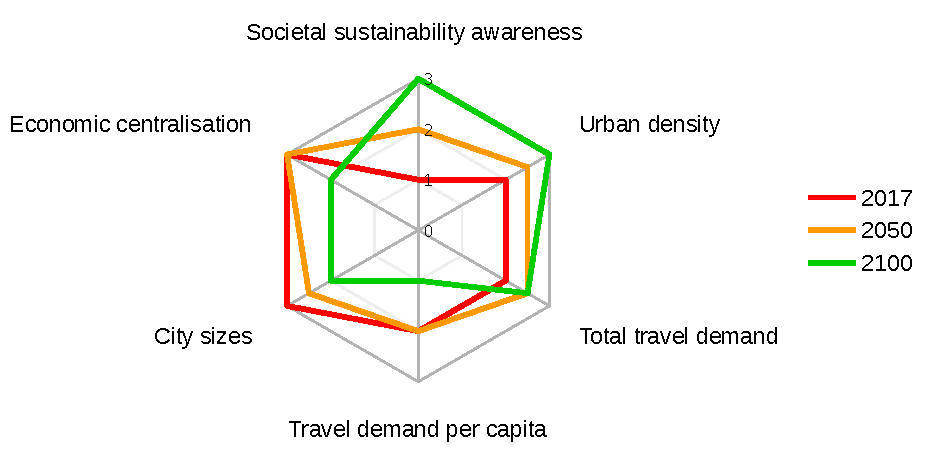
\includegraphics[width=0.8\textwidth]{figures/radar_development-scenario}
\caption[Shifts in development and land-use patterns in SSP1-MOB.]{Radar graph showing the shifts in development trends and land-use patterns found in SSP1 and SSP1-MOB for the years 2100, 2050 and 2017 (baseline). The following values are given to the qualitative variables: 3 for high, 2 for medium and 1 for low.}
\label{f:results:radar_development-scenario}
\end{figure}

\subsubsection*{Cultures of mobility}
As already highlighted in the \sref{ss:results:ssp1-mob-paradigm}, one of the key preconditions for the transition to a sustainable mobility paradigm is a change in the \emph{cultural perception} of mobility (how is it understood). The currently generalised notion of privately owning the means of transportation, namely automobiles, must be challenged if support for public transport is to grow. It is evident that such a challenge goes beyond the culture of mobility, into the general frame of material and ownership cultures. A reduced desire for both private ownership and private freedom of mobility ---which are in opposition to collective ownership and collective freedom--- would also pave the way for car sharing and carpooling schemes, which are currently deemed as lower-status, inconvenient alternatives. Therefore, it is the discourses around personal freedom and private property that must be radically challenged.\todocite{Cite someone?}

Another key aspect of the mobility culture that must be challenged in the future is the conceptual link between movement and (again) the omnipresent discourse on freedom that forms the ideological core of the (neo)liberal society. The mental connection between freedom and freedom of movement must be broken if a reduction in travel demand is desired for the future of SSP1-MOB. The dissociation proves to be difficult, though, since the connection between freedom and mobility is strongly supported by the capitalist economic and ideological framework \parencite{freudendal-pedersen2009_MobilityDailyLife,sheller2012_EmergenceNewCultures}. However, the detachment of mobility from the general concept of freedom is promising from the sustainability point of view; if individual freedom is to emerge from other ``sources'' other than free movement, it is expected that the travel demand per capita gets lower. This is indeed related to the desired reduction of demand in SSP1-MOB, as portrayed in \fref{f:results:radar_development-scenario}.

Particularly, with regards to the most prevalent form of transportation nowadays, the automobile, a lot has to change in its perception from a cultural perspective. If the share of automobile demand has to drop so dramatically as portrayed in SSP1-MOB (from a dominant position to a niche-filing solution), a number of its cultural ``components'' \parencite{urry2004_SystemAutomobility} must be contested and changed:
%
\begin{enumerate}
\item Cars must not be conceived as technological marvels to be worshipped. Instead, they must be understood for what they are: tools for mobility.
\item A change in the value attributions to automobiles is necessary as well, in order to stop it being the second most item of individual consumption, after housing. Values such as freedom, safety, sexual drive or speed must be dissociated from automobiles.
\item Cultural discourses, imagery and symbolic status of automobiles as constituents of the ``good life'' must be contrasted with the impacts that it actually causes; they must be culturally subverted.
\item The subordination of other forms of mobility, such as slow modes, to automobility has to be contested. A new hierarchy of mobilities is needed for a future of denser, bigger and more compact urban areas.
\end{enumerate}

Finally, the shift of cultural perspective must happen not only at the user level, but also at the urban/traffic planner's. \textcite{banister2008_sustainablemobilityparadigm}, drawing from \textcite{marshall2001_challengesustainabletransport}, presents some of the foundation stones of the change to such a sustainable mobility planning paradigm:
%
\begin{enumerate}
\item Instead of speeding up traffic, slowing it down must be the new target for both users and planners.
\item Streets have to be seen as a space for urban life, rather than just public spaces occupied by private automobiles only.
\item Social and environmental multicriteria analyses regarding mobility need to be performed in addition to the already dominant (and only) economic assessments in urban planning.
\item Larger travel \emph{times} for similar or reduced travel \emph{distances} must become acceptable, in contrast to the current ever accelerating pace of society and mobility.
\item In general, attention has to shift from vehicles to people: human, personal mobility should be at the core of the frame, opposed to purely vehicle mobility.
\end{enumerate}

One last remark is worth to be discussed here, with regards to point 4 in the previous enumeration. An important and overseen aspect of sustainable mobility is the different conception of time. Drawing from the analysis that \textcite{zijlstra2012_SocioSpatialPerspective} make about cultural trends that support automobility, \emph{time} has played a central role in modern (capitalist) societies. The concept of time \emph{gaining} is so deeply embedded in modern cultures that acceleration, be it in production lines, communications, shopping activities or, relevantly, transport, has become a paradigmatic goal for almost any development effort in our society. Although not being explicit in the SSP1-MOB narrative, a change of mindset with respect to time is also desirable, since it would flatten the path for slow modes to take over. An example of such a change in lifestyles is already portrayed by \emph{slow cities} \parencite{mayer2006_SlowCitiesSustainable}.

\subsubsection*{Travel mode shifts}
One of the key aspects of the path to SSP1-MOB is travel mode shifting. This is, the relative reduction or increase in the demand share of the various travel modes available until 2100. This shift is visually shown in \fref{f:results:travel-demand-shares}, where the desired shares for 2050 and 2100 are portrayed, in accordance to the estimates given by \textcite{vuuren2017_Energylanduse}.

With respect to the previously discussed components of the backcasted path, culture and land-use patterns are not the only means to achieve the kind of transport mode shift shown in \fref{f:results:travel-demand-shares}. Two more patterns of change are identified in the SSP1-MOB narrative\todonote{Are these patterns really included in the narrative? Intermodal travel might be... Demand management, not so sure! Add it, if necessary!} that should enable faster mode shift rates:
%
\begin{enumerate}
\item Demand management should play a more central role in traffic/urban planning. Following the terminology by \textcite{goodwin2012_ProvidingRoadCapacity}, planning should evolve from a road-centered ``predict-and-provide''\footnote{\textcite{goodwin2012_ProvidingRoadCapacity} originally refers, specifically, to infrastructure (roads/urban) planning approaches.} approach to a truly multi-modal ``predict-and-manage'' perspective. Traffic calming, road and congestion pricing mechanisms, multi-modal demand modelling and public transport facilitating policies (through, e.g., subsidies) should become commonplace in the future, in order to gradually shift travel demand towards the more sustainable transport modes.
\item Intermodal travel must become a reality in the SSP1-MOB world: it is the most prominent way to reduce unsustainable car usage in long-distance trips settings. Automobility is predominant in this type of trips, due to the (perceived) inconvenience of public transport, high costs of non-integrated public transport networks and lack of proper travel information for the end user \parencite{riley2010_IntermodalPassengerTransport}. Therefore, public transport networks must become integrated at much larger scales, with affordable fares and, very importantly, technologies must be developed to convey the necessary information to the users.
\end{enumerate}
 %
\begin{figure}
		\centering
  \begin{subfigure}{0.8\textwidth}
    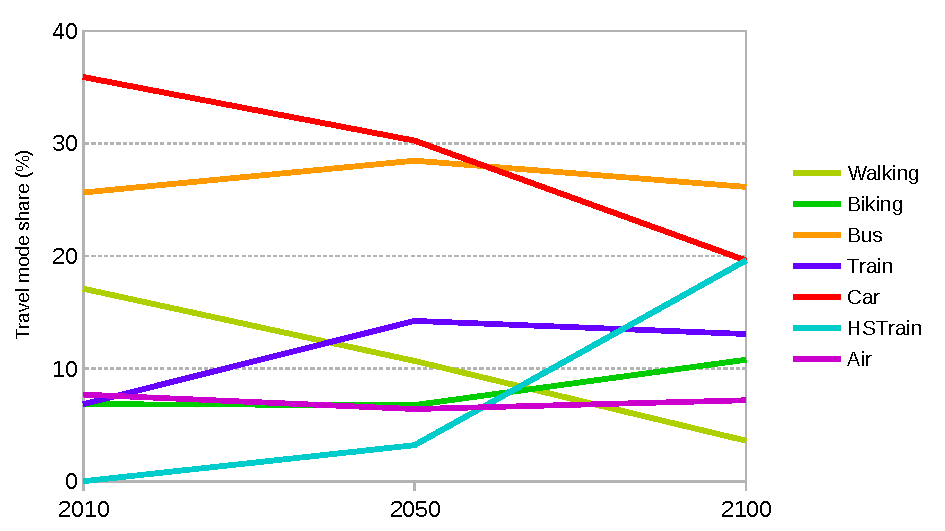
\includegraphics[width=\linewidth]{figures/line_travel-demand-shares.pdf}
    \caption{}
    \label{f:results:line_travel-demand-shares}
  \end{subfigure}
  \begin{subfigure}{0.8\textwidth}
    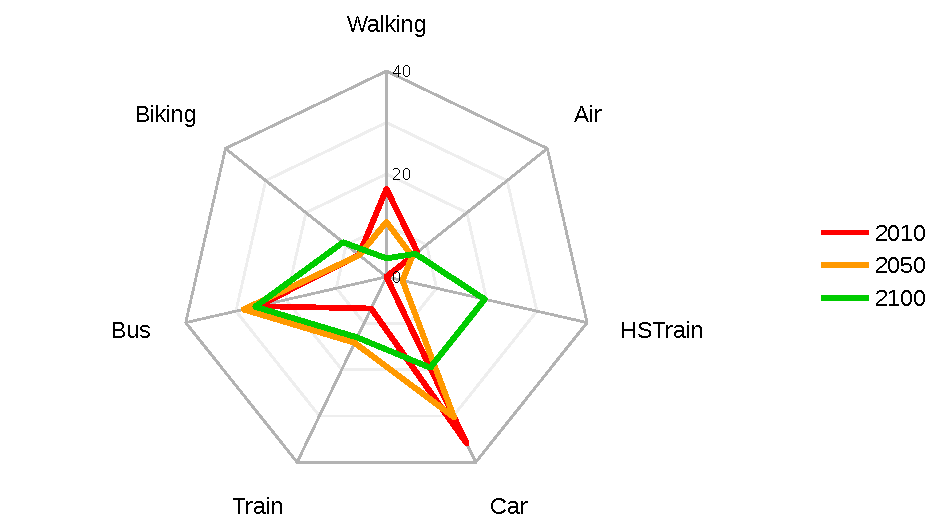
\includegraphics[width=\linewidth]{figures/radar_travel-demand-shares.pdf}
    \caption{}
    \label{f:results:radar_travel-demand-shares}
  \end{subfigure}
  \label{f:results:travel-demand-shares}
  \caption[Evolution and comparison of travel demand shares in SSP1-MOB.]{Evolution (a) and comparison (b) of total travel demand per transport mode (shares), in percentages, across the SSP1-MOB futures and the 2017 baseline. Note: the demand shares are approximated from the figures provided by \textcite{vuuren2017_Energylanduse} in their quantitative appraisal of the SSP1 scenario.}
\end{figure}

\subsubsection*{Vehicle and fuel technologies}
Finally, there is another key category of changes within the transport system that must be tackled in order to follow the path of SSP1-MOB: efficiency increases and technological progress. This applies mostly to the transport technologies themselves: vehicles must be made much more efficient if they are to be run on carbon-based fuels. An extensive electrification of the vehicles is also desired to reach not only low-carbon technologies, but also low-noise, low-emission vehicles that stop polluting the urban areas' air.

With regards to vehicle and fuel technologies, the SSP1-MOB narrative assumes the very high efficiency gains also assumed by \textcite{vuuren2017_Energylanduse} in their implementation of the SSP1 storyline. SSP1-MOB also draws from this implementation the higher share of renewable (bio)fuels in the transport sector and the emergence of hydrogen powered vehicles from 2050 onwards. Needless to say, these technological advances are linked to broader changes in the political and industrial arenas. A political will to devote resources into research and development of key technologies must be developed and, in turn, transport companies must embrace and push for a change in the technological bases of their products.

%%
%\begin{figure}
%		\centering
%  \begin{subfigure}{0.8\textwidth}
%    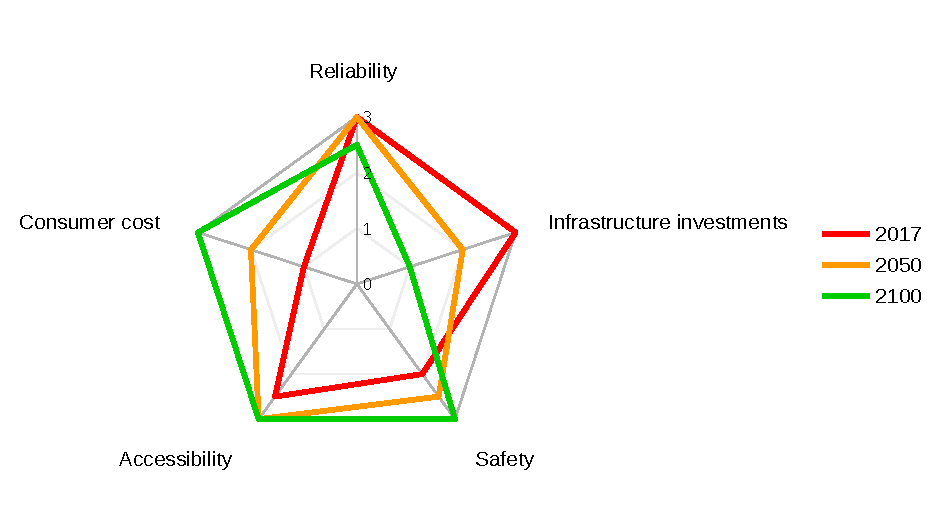
\includegraphics[width=\linewidth]{figures/radar_automobility.pdf}
%    \caption{}
%    \label{f:results:radar_automobility}
%  \end{subfigure}
%  \begin{subfigure}{0.8\textwidth}
%    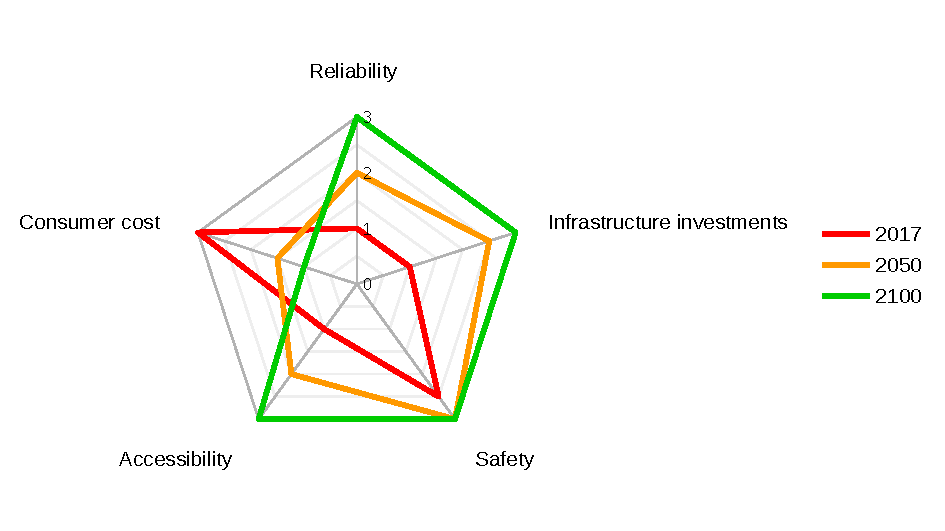
\includegraphics[width=\linewidth]{figures/radar_public-transport.pdf}
%    \caption{}
%    \label{f:results:radar_public-transport}
%  \end{subfigure}
%  \caption[]{}
%\end{figure}

\section[The AUTOLOCK model]{The AUTOLOCK model: understanding the feedback structures that drive the automobility regime}
\label{s:results:autolock-model}
This section is devoted to the investigation of the feedback structure that supports and shapes the system of automobility. \todonote{Perhaps this explanation of \emph{``why cars?''} could be in another chapter: methods? Introduction?}The choice of studying this particular transport mode is based on a triad of arguments: (a) the clear dominance of the automobile as the main mode of transport globally (in terms of travel demand), (b) the huge inertia, complexity and stability that the system has historically posed against threats to its dominance and (c) the fact that this dominance and resilience have become an obstacle for modal shifts, or more generally, a transition to sustainable mobility. Therefore, it is worth it to take a closer look at the dynamics that secure the position of automobility in its current status.

As an example of the automobility resilience, the system has ``survived'' the 1970s oil crisis, the ``dieselgate'' scandal\footnote{``Dieselgate'' refers to the Volkswagen emissions scandal that started in September 2015, when the U.S. Environmental Protection Agency reported that the German automotive industrial group had been faking emission control tests. This caused the \ce{NO_X} output to be lower in the certification tests than in real-world driving scenarios, thus being able to meet U.S. and European emission standards.} \parencite{guardian2017_Volkswagenrevealsrecord}, or even the 2008 global financial crisis. \fref{f:results:global-passenger-car-production} shows the global production of cars from 1961 to 2015, clearly depicting the effects of the financial crisis, whilst acknowledging that production has kept increasing nevertheless.
%
\begin{figure}[h]
\centering
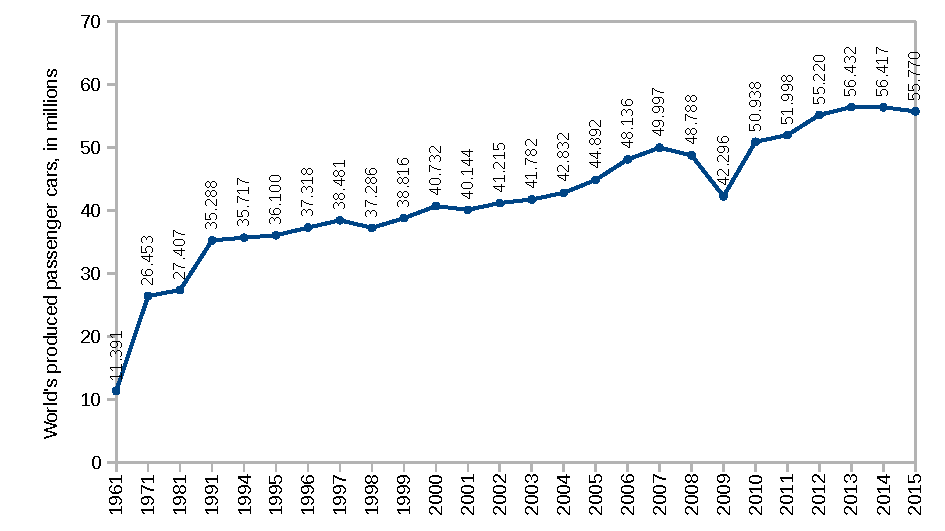
\includegraphics[width=0.85\textwidth]{figures/line_global-car-sales.pdf}
\caption[Global passenger cars production 1961-2015.]{Global passenger car production 1961-2015. Source: own figure; original data from \textcite{bts2017_Table123}.}
\label{f:results:global-passenger-car-production}
\end{figure}

As already mentioned in the \nameref{c:methods} chapter, the study of certain feedback structures of the system, detailed in the following subsections, is carried out through a series of Causal Loop Diagrams (CLD). Because of the resilient nature of the automobility regime, the collection of CLDs that form the overview of the system is referred to as the AUTOLOCK model. \ssref{ss:results:cld_urban-planning} discusses the stability mechanisms of automobility from an urban planning (land use) perspective. Next, the cultural basis and legitimacy apparatus of automobility is described in \ssref{ss:results:cld_cultural-feedbacks}.
% This section was removed Finally, \ssref{ss:results:cld_public-transport-automobility} provides a (partial) explanation of how automobility displaces public transport and vice-versa.

\textbf{Note:} with regards to notation: (a) CLD variables are denoted by a different font face, such as \CLDvar{This Example} and (b) causal loop (\emph{reinforcing} or \emph{balancing}) are denoted by the labels assigned in the diagrams, as in \CLDloop{R1}.

\todoparagraph{(OPTIONAL?)For each of the perspectives studied in the following subsections, a series of \glspl{PLP} are considered. This is, policy intervention is discussed on the basis of where in the feedback structure policy has the potential to be effective, avoiding policy resistance as much as possible.}

\subsection{Urban planning and automobility}
\label{ss:results:cld_urban-planning}
Historically, automobility is linked to the development of road infrastructure on one side and on cultural discourses that legitimise the adoption of private mobility on the other \parencite{goodwin2012_ProvidingRoadCapacity,gartman2004_ThreeAgesAutomobile,sheller2012_EmergenceNewCultures}. \fref{f:results:cld_congestion_1} shows the core reinforcing mechanism of automobility, which is founded on the mobility possibilities it supports, through increased \CLDvar{Accessibility} due to augmented \CLDvar{Road capacity}. Higher \CLDvar{Automobility demand} drives higher \CLDvar{Congestion}, putting pressure for more \CLDvar{Road investments}. \CLDvar{Accessibility}, coupled to a cultural background based on ideals of freedom, is seen as a major enabler for climbing up the social ladder, thus increasing \CLDvar{Automobile ownership} and closing the \CLDloop{R1} reinforcing loop --- the \emph{Automobility freedom} loop. With regards to the \CLDloop{R2} reinforcing loop, it accounts for a well-known rebound effect of motorway capacity expansion: induced travel demand \parencite{hymel2010_Induceddemandrebound,thill2005_Tripmakinginduced}. Most importantly, the cultural framework, represented by \CLDvar{Cultural legitimacy of automobility}, ultimately legitimises and supports these feedback structures.

\begin{figure}[h]
\centering
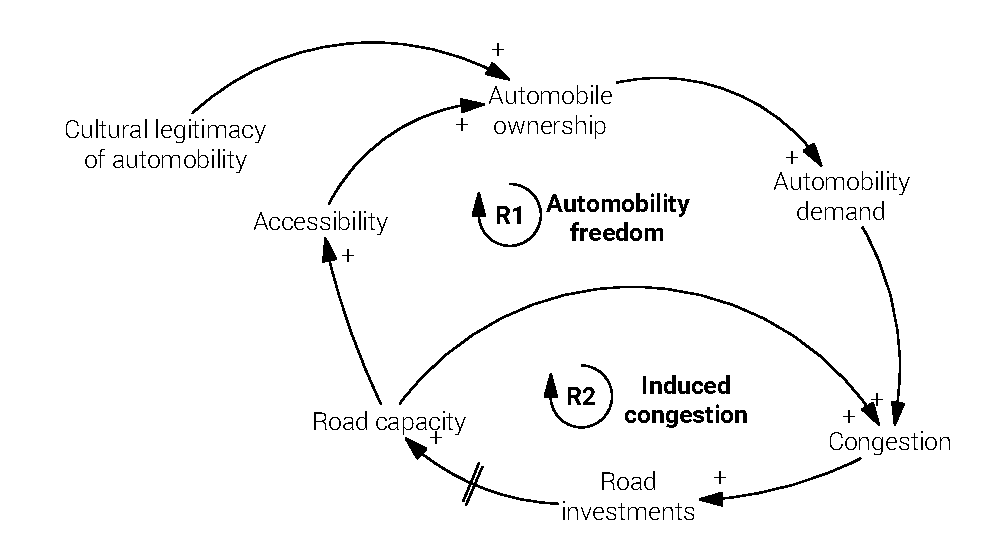
\includegraphics[width=0.7\textwidth]{figures/model/cropped/congestion-urban_1_core.pdf}
\caption{AUTOLOCK socio-spatial perspective: freedom and congestion.}
\label{f:results:cld_congestion_1}
\end{figure}

The increased accessibility provided by the ubiquitous construction (and expansion) of roads, coupled with low fuel/vehicle prices stirs the development of suburbs and causes a focus shift from the planning perspective, from integrated areas towards car-based single-use ones: the \CLDvar{Single-use urban development} variable in \fref{f:results:cld_congestion_2}. \CLDvar{Automobility demand} grows to meet the new requirements derived from the suburban lifestyle, namely the increase in spatial separation of jobs, housing, commercial and recreational areas; in other words, \CLDvar{Average travel distance}. Due to the low population density found in single-use urban developments, public transport becomes infeasible and expensive to maintain. Thus, the automobile rises as the single viable alternative for the residents of the suburbs, closing the \CLDloop{R3} reinforcing loop of \emph{automobility dependence}. This particular feature of the automobile system is particularly relevant for the focus of the present study. Automobility dependence locks in automobile users, planners, developers, etc. within the system practices space and forces them to adapt their lifestyles to this form of mobility \parencite{cullinane2003_Cardependencepublic,koehler2009_transitionsmodelsustainable}\footnote{The concept of \emph{practice space} is used by \textcite{koehler2009_transitionsmodelsustainable} to represent transport alternatives (including automobility) in their modelling and simulation of a sustainable transition.}.

Even though many cities worldwide have begun taking efforts to reduce automobile dependency (and have been doing so for years), it is critical to understand that the existing infrastructure, the huge sunk investments that have been brought into such infrastructure and the overall spatial organisation of residential, commercial and working areas has been built over many decades --- the inertia that these developments have is enormous \parencite{geels2012_AutomobilityTransitionSocio}. Not only because of the large amounts of resources that are needed to re-shape roads, cities and suburbs globally, but because the lifestyle that automobility is tied to has become deeply entrenched in cultural frameworks (as discussed in \sref{s:results:backcasting-ssp1-mob} and \ssref{ss:results:cld_cultural-feedbacks}).

\begin{figure}[h]
\centering
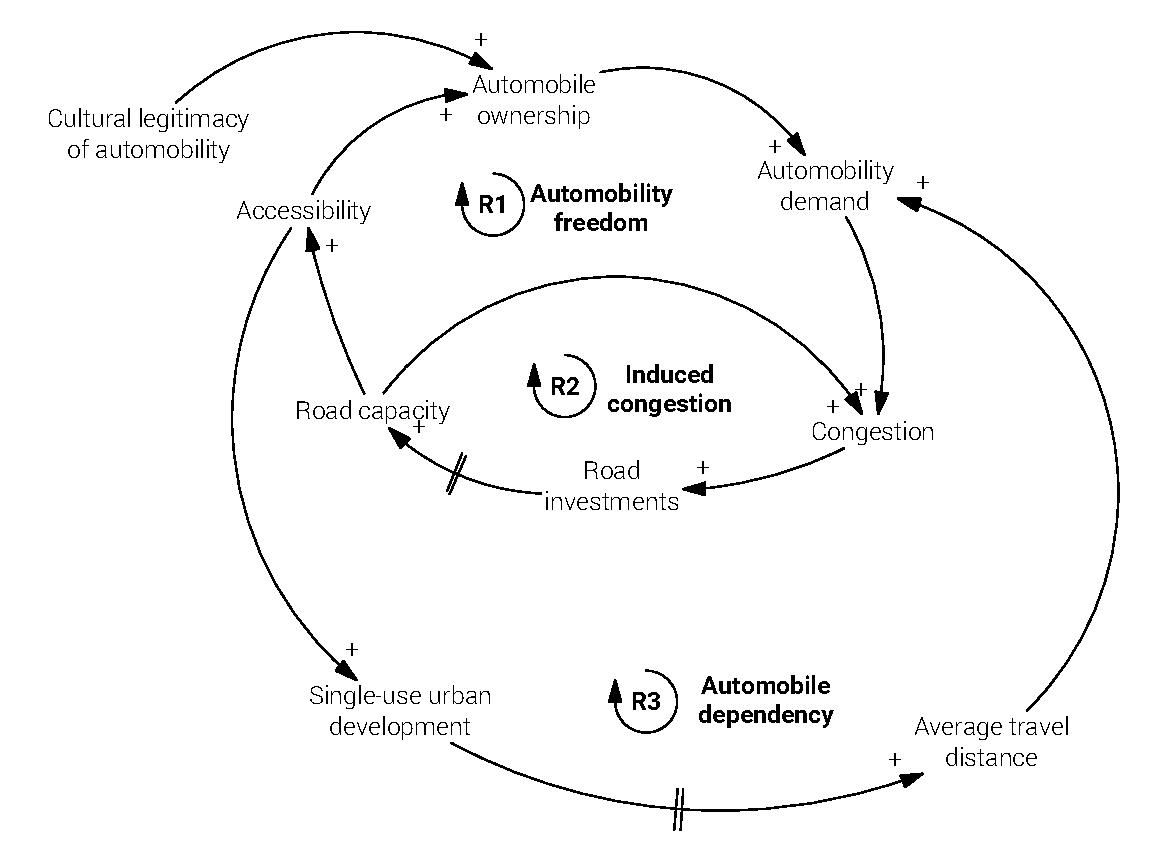
\includegraphics[width=0.8\textwidth]{figures/model/cropped/congestion-urban_2_dependency.pdf}
\caption{AUTOLOCK socio-spatial perspective: building automobile dependence.}
\label{f:results:cld_congestion_2}
\end{figure}

Finally, \fref{f:results:cld_congestion_3} presents additional balancing loops that restraint the further growth of mobility: some of them are endogenous, while some others (\CLDloop{B2} and \CLDloop{B3}) are exogenous\footnote{\emph{Endogenous} refers to dynamics arising from the inner-workings of the system or to actions to support it (single-use planning), while \emph{exogenous} refers to external measures/policies intended to counteract automobility use.}. For instance, \CLDvar{Average travel time} is an important factor contributing to the perceived accessibility that automobiles provide. If, due to congestion or longer travel distances, the time spent is excessive, the user might not find it convenient (accessible) to drive around. \CLDloop{B1} captures this phenomenon. When \CLDvar{Demand management policies} (e.g., road pricing) are introduced, another balancing feedback is produced, creating the \CLDloop{B2} loop \parencite{banister2008_sustainablemobilityparadigm,dudley2012_DynamicsRegimeStrength}.

Furthermore, the use of \CLDvar{Mixed-use urban development} techniques reduces, with time, the \CLDvar{Average travel distance}, thus alleviating the pressure on \CLDvar{Automobility demand}, portrayed in the \CLDloop{B3} balancing loop. However, the mutual exclusivity between mixed and single-use development patterns found in many regulatory frameworks \parencite{hirt2007_DevilIsDefinitions} means that they are in direct competition: if one planning practice increases, the other decreases and vice-versa. This feature is captured by the reinforcing loop \CLDloop{R5}. Finally, in a similar fashion to \CLDloop{B1}, another balancing force opposes the absolute dominance of automobiles: if suburbs grow in size and extension, not only time, but \CLDvar{Average travel distance} increases, thus reducing the perceived \CLDvar{Accessibility}, giving rise to \CLDloop{B4}.

\begin{figure}[h]
\centering
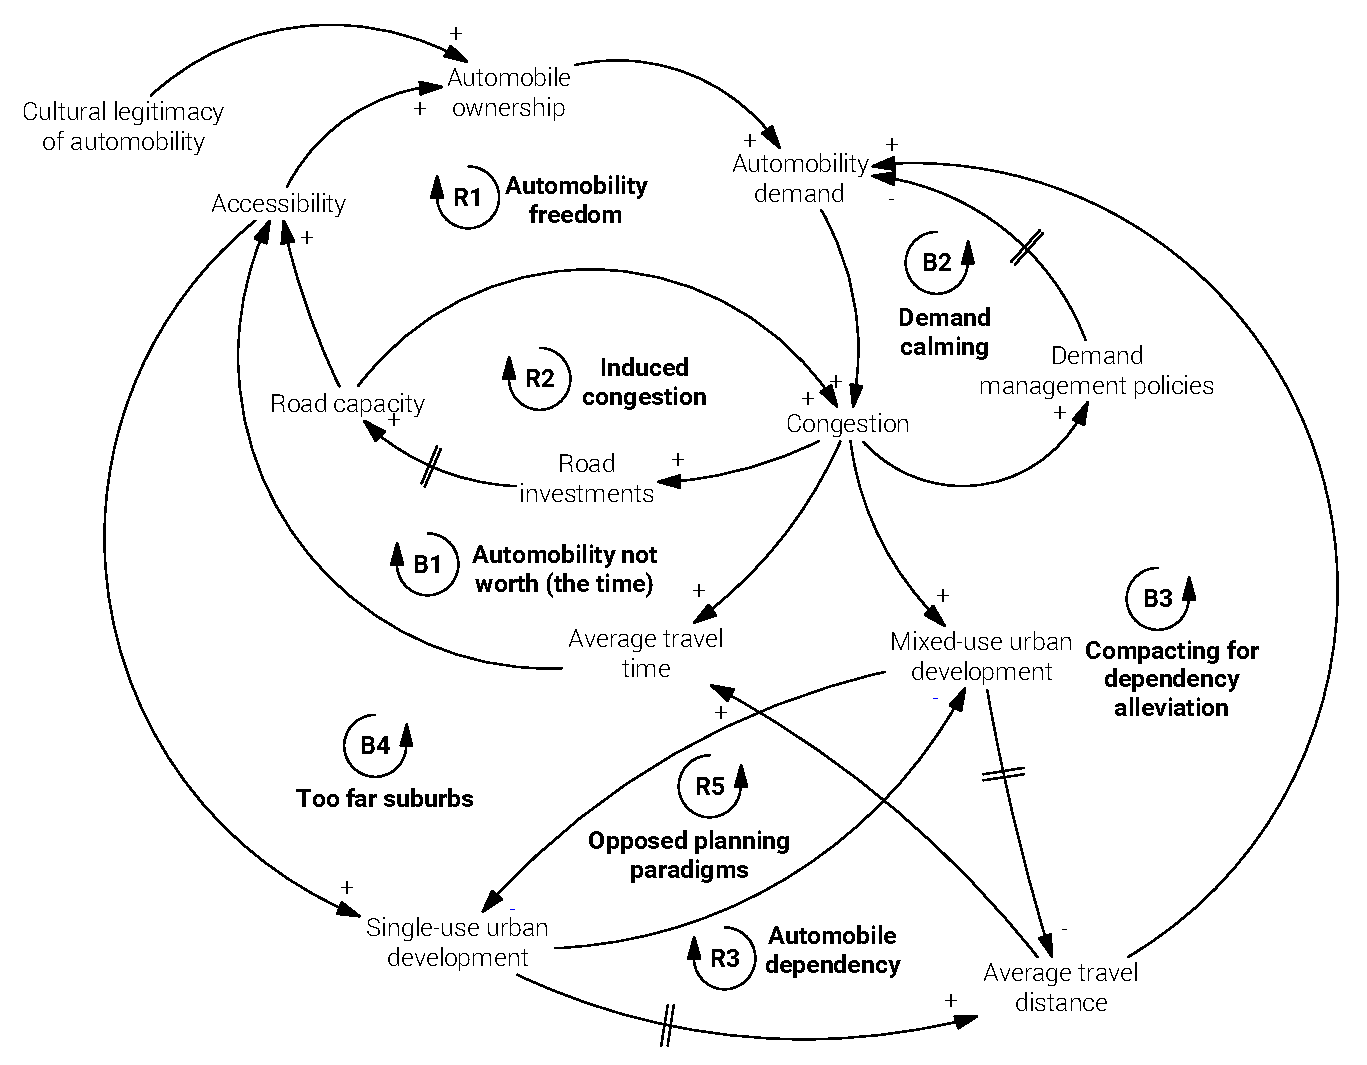
\includegraphics[width=\textwidth]{figures/model/cropped/congestion-urban_3_final.pdf}
\caption{AUTOLOCK socio-spatial perspective: balancing forces.}
\label{f:results:cld_congestion_3}
\end{figure}

\subsection{Cultural legitimacy feedbacks}
\label{ss:results:cld_cultural-feedbacks}
A highly relevant issue to discuss, with respect to the cultural dimension of automobility, is the legitimacy apparatus that supports it and, at the same time, dis-legitimises other forms of mobility (public transport, cycling, etc.). Due to the limitations in the scope of this study, only this central aspect will be analysed, since the range of practices and discourses that form the body of the automobility culture is huge. Therefore, this subsection is aimed at revealing the dynamics behind the \emph{acceptance} of automobility as a cultural reality.

\fref{f:results:cld_culture_1} draws from the CLD diagram in the previous section. The core reinforcing mechanism that drives \CLDvar{Automobility demand} growth (\CLDloop{R1}), is based on the \CLDvar{Cultural legitimacy of automobility}. However, unlike the CLD model in \ssref{ss:results:cld_urban-planning}, cultural legitimacy is not an external (supporting) force, but rather an integral part of the \emph{Freedom to move} discourse that sustains \CLDloop{R1}. The \CLDvar{Automobility capacity} variable is meant as the user's perception of the potential to access more destinations (accessibility) through better, uncongested roads (road capacity). Therefore, \CLDvar{Automobility capacity} is directly and proportionally linked to cultural legitimacy, since the perception of a higher ``degree of freedom'' reinforces the belief (the legitimacy) that automobility is the \emph{right} alternative to choose. However, there is a clear precondition that must hold to support this legitimacy dynamic: an framing \CLDvar{Discourse on individual freedom} as the highest (moral) value in the values hierarchy \parencite{urry2004_SystemAutomobility,boehm2006_PartOneConceptualizing,sheller2008_MobilityFreedomPublic}.

Secondly, \fref{f:results:cld_culture_1} shows another reinforcing loop, \CLDloop{R2}, that also contributes to increasing the \CLDvar{Cultural legitimacy of automobility}. It does so by providing the necessary lifestyle satisfaction (beyond the realisation of \emph{freedom}). Increased \CLDvar{Automobility capacity} enables the fulfilment of activities that (have) become embedded in the lifestyle: practices such as commuting, car-based grocery shopping, chauffeuring family members, weekend and holidays car-based tourism, etc. It is then important to understand that a lifestyle is a meaning carrier. Lifestyles are used to express one's identity, a ``narrative of the self''. Lifestyles are made of behaviours, conducts and practices that are adopted beyond their utility: they shape the individual's identity \parencite{giddens1991_ModernitySelfIdentity,spaargaren2000_Lifestylesconsumptionenvironment}. \CLDvar{Lifestyle satisfaction} then becomes the main mechanism to achieve a \CLDvar{Sense of individual identity} \parencite{ropke1999_dynamicswillingnessconsume}, closing the \CLDloop{R2} reinforcing loop, labelled as \emph{Seek for identity}.

\begin{figure}[h]
\centering
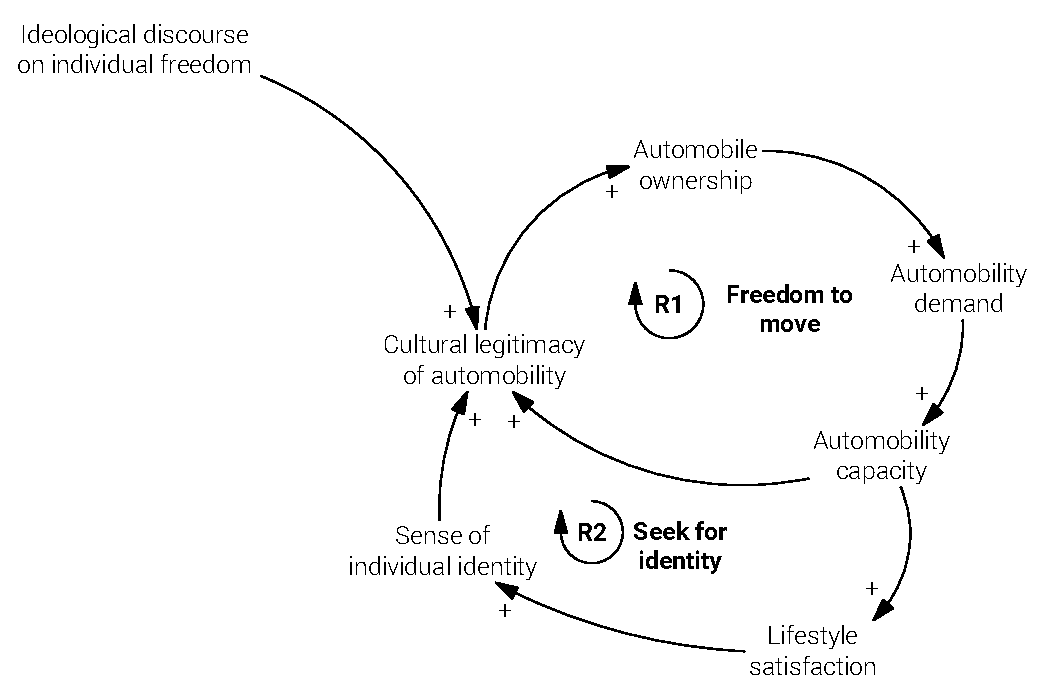
\includegraphics[width=0.7\textwidth]{figures/model/cropped/cultural_1_core.pdf}
\caption{AUTOLOCK cultural legitimacy perspective: identity and freedom.}
\label{f:results:cld_culture_1}
\end{figure}

\fref{f:results:cld_culture_2} adds an important feature of automobility: cultural homogenisation. \textcite{gartman2004_ThreeAgesAutomobile} argues that, similarly to other mass-manufactured products in the capitalist regime, automobiles have become yet another force of cultural homogenisation (\CLDvar{(Auto)mobility homogenisation}). This effect of the industrialisation of automobiles production, which holds especially during the Fordist era\footnote{Fordism refers to the application of manufacturing processes in the industry, following the example of Henry Ford. These techniques consist, in essence, of large-scale and highly mechanised production.}, leads to a decreased \CLDvar{Sense of individual identity}, since the ownership of an automobile no longer distinguishes an individual from another (everyone owns a car). This effectively closes a balancing loop, \CLDloop{B1}, where the loss of individuation power of automobility causes shrinking (or stagnant, at least) auto-ownership and demand.

As a response to the previous effect, the automotive industry has developed a new production pattern: a much wider range of automobile types (e.g., SUVs\footnote{SUV stands for \textit{S}port \textit{U}tility \textit{V}ehicle or \textit{S}uburban \textit{U}tility \textit{V}ehicle.}, hybrid cars, minivans, familiar vehicles, sportive cars, etc.) is offered to the users, with the intention to reach to lifestyle niches, that soon become mainstream markets on their own \parencite{gartman2004_ThreeAgesAutomobile}. This response proves to be effective, further accentuating the \CLDvar{Subcultural division} and, thus, satisfying the need for a \CLDvar{Sense of individual identity}. This mechanism is labelled in \fref{f:results:cld_culture_2} as the \CLDloop{R3} reinforcing loop of \emph{Cultural distinction}.

\begin{figure}[h]
\centering
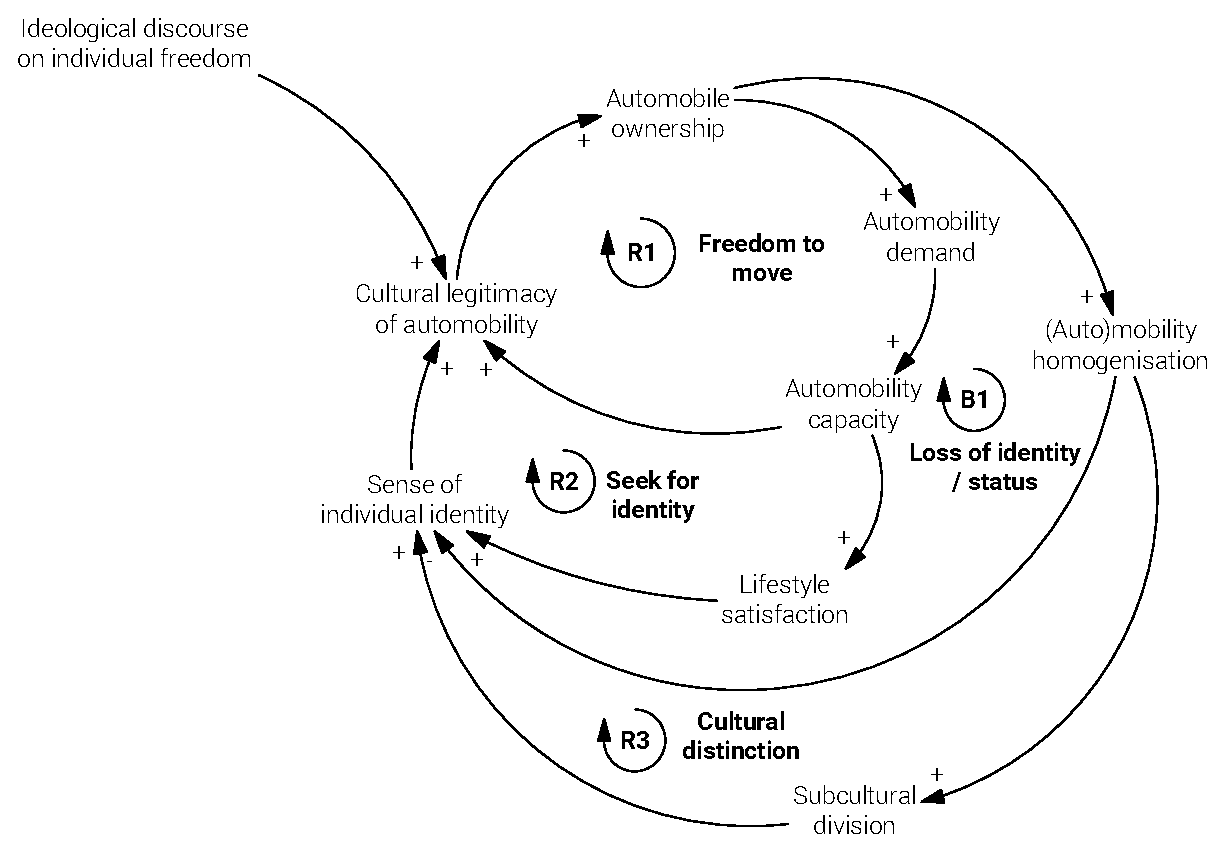
\includegraphics[width=\textwidth]{figures/model/cropped/cultural_2_subcultures.pdf}
\caption{AUTOLOCK cultural legitimacy perspective: homogenisation and subcultural division in (post)modernity.}
\label{f:results:cld_culture_2}
\end{figure}

\fref{f:results:cld_culture_3} incorporates a \emph{critical theory}\footnote{The \emph{critical theory} refers to the philosophical approach used by the scholars in the Frankfurt School to discuss issues such as the critique of capitalist societies, the modernities or the pursue of social emancipation.} approach to the analysis, investigating the origin of the \CLDvar{Need for individuation} that drives the legitimated institution of automobility as a integral component of the culture. The core of this analysis is the reinforcing loop \CLDloop{R4}, labelled \emph{Capitalism}, in which the concepts of \CLDvar{Socio-economic heteronomy}\footnote{\emph{Heteronomy}, in contrast to \emph{autonomy}, refers to the state in which an individual's actions are driven by forces external to itself. This is, heteronomous are those that are ruled by others. Note that, in the context of this study, the emphasis is put in the socio-economic aspect of heteronomy: the impossibility to conduct a lifestyle due to economic and social constraints (e.g., poverty, class conflicts, dominance/oppression relations, etc.).} and \CLDvar{Individual autonomy}\footnote{\emph{Autonomy} refers to the ability of an individual to be self-determined and self-governed.} are opposed. In the capitalist economy, class relations ultimately dictate the level of (socio-economic) autonomy an individual has. By not owning the production means, workers are highly heteronomous and bound to the forces of the labour market, social safety nets and other supra-individual institutions. In this context, due to the lack of \emph{political} \CLDvar{Individual autonomy}, identity is sought in \emph{cultural} individualisation (\CLDvar{Need for individuation}) \parencite{gartman2004_ThreeAgesAutomobile}.

\begin{figure}
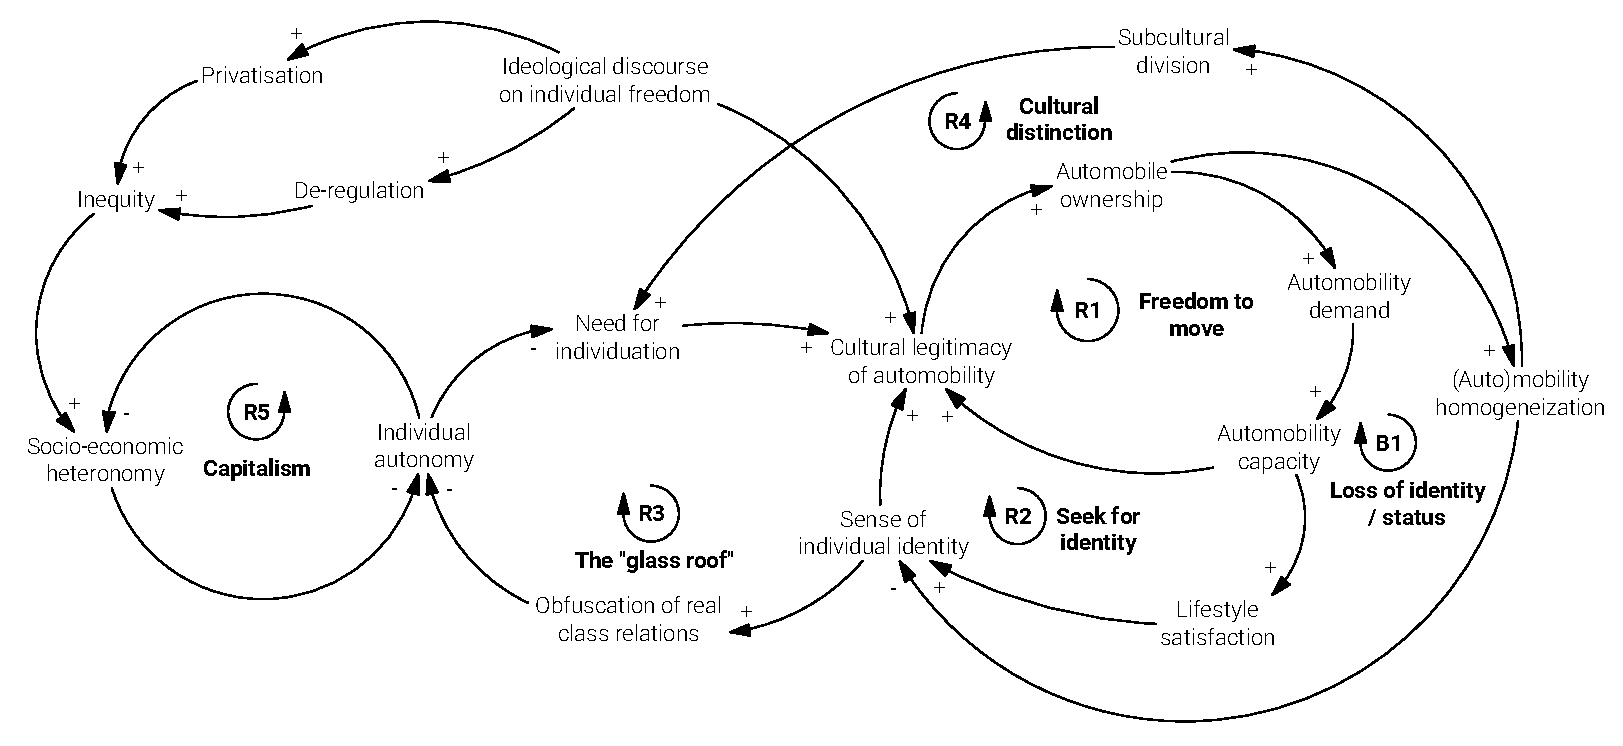
\includegraphics[width=1.2\textwidth,center]{figures/model/cropped/cultural_3_final.pdf}
\caption[AUTOLOCK cultural legitimacy perspective: class relations.]{AUTOLOCK cultural legitimacy perspective: class relations in neoliberal capitalism -- autonomy and heteronomy.}
\label{f:results:cld_culture_3}
\end{figure}

Further deep in the discussion about identity, individuality and autonomy/heteronomy, postmodernist\footnote{TODO} scholars claim that \CLDvar{Subcultural division} liberates individuals from class struggles. The liberation is due to the fact that identity is expressed within a subculture that is not necessarily superior to any other --- i.e., there is no hierarchy, no class \parencite{gartman2004_ThreeAgesAutomobile}. Under the postmodernist perspective, the automobile becomes a liberating product, with its capability to support many lifestyles.

However, the argument held by postmodernist scholars is a highly controversial one. Critical theory provides a very different explanation for the apparent relaxation of class conflicts in the late-capitalism era of mass consumption. The compensatory individuality sought in mass consumption (in automobility, in this study) to alleviate the deprivation of economic autonomy is not liberating. Instead, the mass consumption culture acts by hiding the real class relations: everyone, from all social classes, participates in the same consumption culture \parencite{gartman1991_CultureasClass,marcuse2013_OneDimensionalMan}. The boundaries of classes become diffuse in appearance and the (capitalist/automotive) culture becomes legitimised \parencite{gartman2004_ThreeAgesAutomobile}. These dynamics are presented in \fref{f:results:cld_culture_3} as the \CLDloop{R6} loop (\emph{The ``glass roof''}), which represents the hidden class relations that ultimately reinforce \CLDvar{Socio-economic heteronomy}. Also, the link from the \CLDvar{Need for individuation} variable to \CLDvar{Individual autonomy} is \emph{dashed}, to signify the postmodernist ``liberating'' individuality that subcultures produce, which is actually non-existent according to critical theory. 

Finally, a connection is depicted in \fref{f:results:cld_culture_3} from the overarching \CLDvar{Ideological discourse on individual freedom} to \CLDvar{Socio-economic heteronomy}, where (economic) \CLDvar{Inequity}, preceded by \CLDvar{Privatisation} and \CLDvar{De-regulation}, acts as the mediating mechanism. Following \textcite{monbiot2016_Neoliberalismideology,klein2008_shockdoctrinerise} analyses, the fundamentalist defence of unfettered (individual) freedom, comes at the expense of social/state interventions. The radical market ideology of neoliberalism is based on three tenets: \CLDvar{Privatisation}, \CLDvar{De-regulation} and free trade. It is now widely recognised that this ideology has brought huge increases in inequality during the last decades \parencite{milanovic2016_GlobalInequality,piketty2014_CapitalTwentyFirst}. Inequality is, precisely, the main source of \CLDvar{Socio-economic heteronomy}.

%\subsection{Public transport vs. Automobility}
%\label{ss:results:cld_public-transport-automobility}
%\todowarning{Is this section even necessary? What does it convey? Is there a way to incorporate stuff into the first CLD?}
%\begin{figure}[h]
%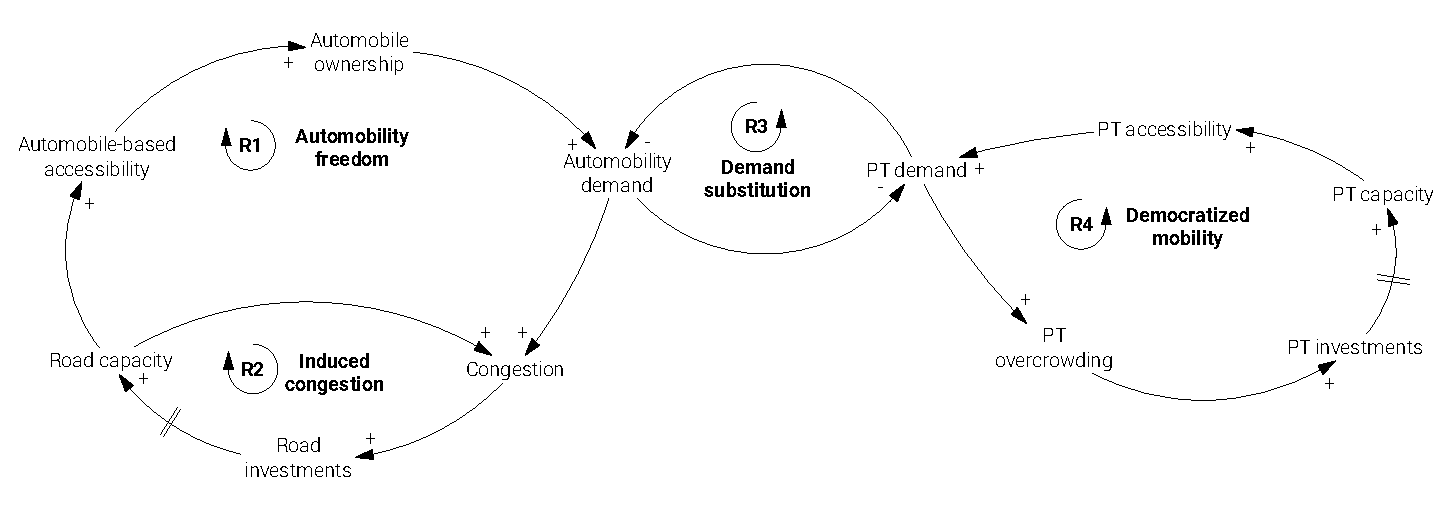
\includegraphics[width=1.1\textwidth,center]{figures/model/cropped/public-transport_1_core.pdf}
%\caption[]{}
%\label{f:results:cld_pt_1}
%\end{figure}
%
%\begin{figure}[h]
%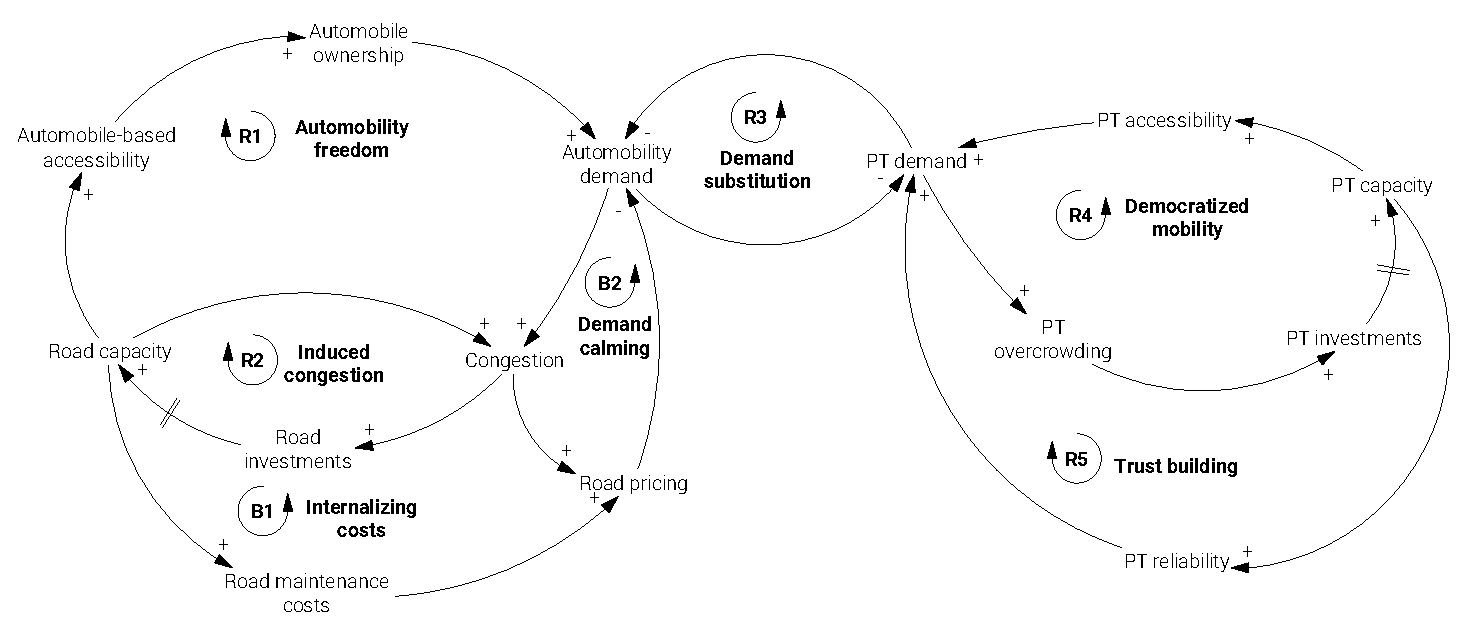
\includegraphics[width=1.1\textwidth,center]{figures/model/cropped/public-transport_2_trust.pdf}
%\caption[]{}
%\label{f:results:cld_pt_2}
%\end{figure}
%
%\begin{figure}
%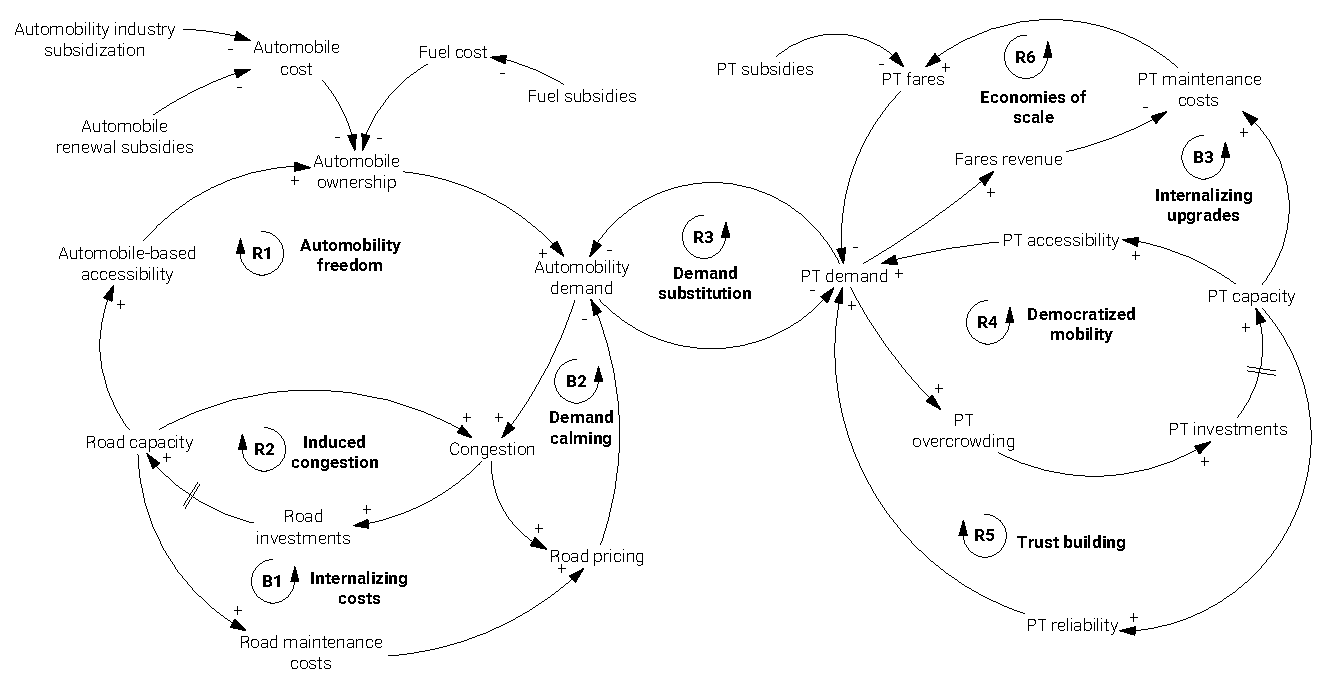
\includegraphics[width=1.2\textwidth,center]{figures/model/cropped/public-transport_3_final.pdf}
%\caption[]{}
%\label{f:results:cld_pt_3}
%\end{figure}

\section[Transition-oriented policy recommendations]{Transition-oriented policy recommendations for a future sustainable mobility}
\label{s:results:policy-recommendations}
% (Geels et al, 2012)
% The logic of the MLP suggests policy makers can follow two strategies
% to influence transitions:
%   i) Enhance pressure on regimes through economic instruments and regulation
%  ii) Stimulate the emergence and diffusion of niche innovations
This final section of the Results chapter covers the ultimate goal of the thesis: deriving \gls{PR} for a transition to a sustainable mobility future\footnote{Some of the recommendations are more indeterminate than others, due to the uncertainties and broad spectrum of the policy targets, e.g., niche promotion policies (specific niches are unexpected).}. A transitions oriented approach backs the suggestions, which are categorised into \emph{niche} (\ssref{ss:results:policies_niche}), \emph{regime} (\ssref{ss:results:policies_regime}) and \emph{landscape} level policies (\ssref{ss:results:policies_landscape}). Target audiences for the \glspl{PR} are given too, since some of them require international governance cooperation and some others are suited to local administrations. Finally, the transitions theory MLP approach suggests two general directions that policy makers can follow to induce the required changes for a transition: (a) put pressure on the regimes via legislation, regulation and economic instruments and (b) stimulate socio-technical innovations at the niche level \parencite{kemp2007_Transitionmanagementas,geels2012_AutomobilityTransitionSocio}.

\subsection{Niche level policies}
\label{ss:results:policies_niche}
Niche level policies are based on the assumption that forecasting the emergence or success of socio-technical niches to overthrow regimes is difficult or even impossible. However, following the scholarship of \emph{transition management} studies, policies can be put in place to, for example, ensure that already existent niches are guaranteed a safe space to develop \parencite{kemp2011_TransitionManagementas}. To do so, protection could be provided until the socio-technical niches gain enough momentum to compete against the regime (through competition agencies at the national or international level). Local, regional, national or international agents such as governments or private initiatives should also guarantee enough funding, through investment programmes, so that niches can sustain their radical innovation process.

With regards to the financing option, not only direct investments can be granted to specific actors within a niche: research initiatives at universities or institutes or even at private companies should be reinforced, especially those that pose to be promising in debunking existing regimes. This way, already in-place niches can be further developed and new niches can emerge. Special care should be taken for niches that go beyond technological improvements (such as battery electric vehicles). Initiatives that build counter-cultural movements (contrary to the established unsustainable mobility culture) should be promoted by the authorities. At the same time, these institutional agents should set a common vision for the kind of sustainable mobility they desire (across governance levels) and, most importantly, have the will to follow it and definitively distance themselves from the current regime.

One last comment is worth making with regards to niche-supporting policy: there is a strong need for policy makers to research the niches eligible of support and to understand the mechanisms of innovation that drive them. Furthermore, there is an urgent necessity of policy coordination and of a disassociation from opportunistic and fragmented policy programmes that serve political agendas\footnote{\emph{Political} is used here in reference to \emph{politics}, which differs from \emph{policy}. Politics deals with power struggles in government, while policy is the consistent set of actions and methods that orient current and future decisions.} \parencite{kemp2004_ManagingTransitionSustainable}.

\subsection{Regime level policies}
\label{ss:results:policies_regime}
Considering SSP1-MOB as the desired vision for mobility, a two-fold strategy is recommended by this study to policy makers in order to achieve a successful sustainable transition. First of all, it is clear that support for the current automobility regime must be dropped significantly. Secondly, public transport must be increasingly supported as the alternative regime that competes with automobility.

At the local level (municipalities), reducing car usage can be achieved with the introduction of, for example, congestion taxes\footnote{Congestion charges have been successfully applied in London and Stockholm, Gothenburg, Durham, Valletta and Milan, in Europe.}. Other subtler measures for traffic calming include the design of road networks that impede or obstruct automobile transit\footnote{The city of Pontevedra introduced such mechanisms, reaching a record low level of automobility \parencite{precedo2017_Pontevedraelsueno} and the city of Barcelona is experimenting with ``super-aisles'', where chunks of streets become isolated from regular traffic (only pedestrians, cyclists and neighbours can access the blocks), hindering the convenience of automobility \parencite{ajuntamentbarcelona2016_OmplimdeVida}.} and the decision to change urban use planning towards a more mixed use pattern that promotes lower mobility. Furthermore, local authorities should reinforce their commitment with public transport by investing even more in building a safe, reliable and convenient network.

Regional authorities carry the responsibility to manage large scale urban and infrastructural developments. Therefore, it is the most suitable locus for integration efforts of local public transport networks, as well as increased funding and subsidisation of this alternative regime. An integrated public transport network at the large scale is a fundamental requirement to advance in the transition path to SSP1-MOB --- regular and high-speed railways are part pf such a network, as are inter-city bus lines, for example. Cheap, long-distance public transport should be a central focus point of regional mobility policy. Moreover, in order to weaken automobility dominance, land use patterns at a broader scale can be adjusted to cut down on suburban sprawl, avoid inter-territorial (between municipalities) single-use areas that encourage car dependency and the like.

Finally, national governments, agencies, and international governance institutions should lead the transition to sustainable mobility by finishing, once and for all, the apparently symbiotic relationship they have with the automotive industry \parencite{wells2012_TransitionfailureUnderstanding,sturgeon2009_CrisisProtectionAutomotive}. Economic rescues should not be a political priority, if the regime is to be challenged. Moreover, fuel subsidies and car renewal (``scrappage'') programmes should also be left behind. Stringent emission regulations should be issued with increasing pressure in the emission levels themselves, in the compensatory taxes and by shortening the time frames for technological improvement. On the other side, high education curricula of infrastructure engineering or urban planning should include a strong focus on sustainability and sustainable mobility in particular, in order to accelerate the pace of the transition at the theoretical and practical levels.

\subsection{Landscape level policies}
\label{ss:results:policies_landscape}
The socio-technical landscape level seems difficult to influence through policies because of its definition as a broad social context where beliefs, ideologies, societal values, concerns, macroeconomic trends, infrastructure or media are included. However, some of these aspects can effectively be targeted by policies, perhaps at the national and international level. Carbon taxes are an example of such policies, in that they induce innovation in the automotive industry by indirectly orienting their research efforts to cleaner technologies \parencite{aghion2016_CarbonTaxesPath}. These type of taxes should be applied at the international level, or at least be coordinated in such spaces. Further examples of policy instruments to address sustainability in transport, beyond automobility, are international aviation taxes, emission trading for airline companies or levies on air-borne emissions \parencite{peeters2006_Innovationtowardstourism}.

Another form of landscape-level policy that complements economic instruments like the ones cited before is betting for an integrated, efficient and reliable (inter)national public transport network. High speed trains, either national or connecting several countries, should be put in place, due to their higher energy, land-use and social ``efficiency''. Strongly linked to transport infrastructure efforts, the aforementioned electric grid expansion (in size, but also in international integration) and the decarbonisation of the energy system are also landscape developments that would push for sustainable mobility. The policy recommendation in this case is to invest and promote investments in such areas, as well as passing regulations that force the necessary transition to renewable energy sources onto the private energy sector. Phasing-out fossil fuels is also mandatory for putting pressure on the automobility regime, as well as for transitioning to the energy system that SSP1-MOB relies on --- (economic and political) incentives should be put in place for the development of bio-fuel, electric battery and hydrogen fuel cell technologies.

Finally, with regards to the cultural and ideological aspects of the mobility landscape, a lot of work is still ahead in terms of policy. If the dominant neoliberal ideology is not challenged also from the political standpoint, it is unlikely that a fast sustainability transition takes place in the near-mid future. Unless the individualist and \emph{laisez fare} tenets held by market fundamentalists are de-legitimised, through cultural but also policy mechanisms, consumption patterns will not change, industries will keep business as usual and sustainability will not be a concern --- most of the pressing issues deal with impacts to the \emph{commons}, that are not recognised by free market fanatics \parencite{kumi2014_Canpost2015,cervantes2013_IdeologyNeoliberalismSustainable}. Therefore, if sustainability is the truly desired goal for human development, neoliberal policies and all the discourses that underpin them must be left behind in policy schemes.